\section{The Story}% {{{
\label{sec:the_story}

\subsection{Coma}%
\label{sub:coma}

\subsubsection{Getting to know the characters}%
\label{ssub:getting_to_know_the_characters}

The goal of this scene is to give each player a few minutes to get to know their own character, and build some “memories”, such
that they could start the first group scene with more confidence.  In addition this scene will be giving them someone to lose
and/or care about in the world when they are brought into \textbf{Inferno}.

This scene is a one on one scene, so if you're playing face to face, ask them to sit in a chair opposite of you for the
duration of the scene; or if you're playing online ask all the other players to turn off their camera, to make the scene feel
more intense and intimate.

The scene starts with the character in coma, they don't need to know how they got in it.  The important fact is that they are
here, and with them is their important relationship who is visiting regularly, how regular is not important.  Tell the player
that because they know each other so well, as if by magic their relationship can hear their thoughts as if they were speaking
out loud.  A lot of this scene will be improvising on the spot.

If you have time enough (4h or more) this should have the following arc:
\begin{enumerate}
  \item Roll to~\bluebf{Keep it together (+Willpower)} to see how much their time in a coma has worn down their stability.

  \item The relationship tells about their current life, events that have happened in the last week, maybe small problems turn up.

  \item The relationship tells of something exciting happening, here get creative the only thing to avoid is things like a
        lottery win or other gain of wealth, because it will work against one of the goals of the introductory section to make the
        decision to accept the experimental treatment a bit more convincing.  For example things that I used were a gay couple going
        through with their adoption, a mother finding a good new potential partner, who is treating them well, sister going from doing
        bad at school to discovering a new subject that they are really good at.  This high is meant to make the next bit more dire.

  \item Since this is set in a US hospital the costs of being in there are ramping up, and for the scientist a promising new
        grant could be gotten, and similar for the careerist a new contract is in sight, if they were there to help the other
        (incompetent) team members to get that.  In essence there is the need to wake up, rather sooner than later.

  \item Last bit is to present them with a consent sheet that their relationship found or someone called in a last big favour
        to get them on an experimental treatment program, or blackmail by their relationship of the doctors here, are just a few
        examples.  Names like Joanna O'Banion\index{O'Banion, Joanna} and her expertise can be dropped, but all interactions are
        with her assistants or other doctors in this department.

  \item Ultimately the sheet is signed or the patient is put on the experimental program through favours, bribing, blackmailing
        depending what the character or rather their relationship is willing to do.

  \item After that the character is brought to the 5\textsuperscript{th} by a brutish looking orderly, with dirty fingernails
        smelling of ashes and mould.  The room (504) slowly fills with all the player characters.
\end{enumerate}

\gmnote{%
  If one of your players decides to convince their relationship to mercy-kill them, then that is perfectly fine.

  That player wouldn't wake up in the shared “wake-up room”, but in a room next door as a ghost, being able to see though walls
  as if they were semi-transparent, like frosted glass.  Dying and waking up from the dead as a ghost is a traumatic experience,
  so they loose \redbf{-2 Stability} and if the GM sees fit they gain the following disadvantage.
}

\paragraph{\(\diamond\)~\index{Disadvantages!Cannibalism}Cannibalism}\label{disadv:cannibalism}%
You have an unnatural hunger you crave for human meat whenever you see an open wound or organs roll \bluebf{Disadvantage (+0)}.
\begin{description}
  \item[(\KULTred{15+})] You are in check of your hunger, you can control it and not the other way around.
  \item[(\KULTred{10--14})] You control your hunger, but you reveal some of your urges.
  \item[(\KULTred{-9})] Your hunger is overbearing you chomp down on the feast in front of you.
\end{description}
\KULTrule%

This set of scenes is something all my players have highlighted as very intimate and enjoyable, so I wouldn't skip this.

\subsection*{Optional: wake up timer}
If you want to hone in on the impending doom and hammer home that this game is on a timer, you can periodically “broadcast”
nightmares and visions triggered by Dean Moran's\index{Moran, Dean} waking by Joanna, who is now rushing to do the same ritual
with Dean as she did with our lovely PCs.

\subsection{Wake up}%
\label{sub:wake_up}

After the patients have been brought up to the ward, there is a drastic change in tone.  The visitations of their close relations
stop visiting triggering another~\bluebf{Keep it together (+Willpower)} roll, as this should feel like a significant loss.

Instead of them a pale faced, Italian looking lady in white coat and a name tag reading Dr.~O'Banion.  She experiments on them
noting the results in \hyperref[notebook]{a worn notebook}~(p.~\pageref{notebook}). Those experiments are inhumane, suffocation,
cutting, electrocution, and tattooing something on their backs. Note that the protagonists are unable to see or everything in
detail so the smell, sound, and other sensations should give a some horror of not knowing exactly what happened. The protagonists
can later learn about this in the patient files at the foot of their beds.

\subsection{Exploration}%
\label{sub:exploration}

The constant experimentation of Joanna O'Banion\index{O'Banion, Joanna} has brought the 5\textsuperscript{th} floor of Chicago
central hospital very close to \textbf{Inferno}~\cite[p.~314]{KULT:core}.  By successfully waking up the protagonists the floor
is now completely embedded in \textbf{Inferno}, she has managed to seal the floor off to its denizens, by barricading all
entrances and exits but those barriers are unstable and “glitchy”.

In general the \textbf{Illusion} in the ward is thin enough that if you try to \bluebf{See Through the Illusion} you see back
into “Reality”, and you can see the mundane life in a regular hospital, or just hear muffled sounds or smells on a success with
complications.

\subsubsection{Wake-up room: 504}%
\label{ssub:wake_up_room}

\begin{figure}[!htbp]
  \centering
  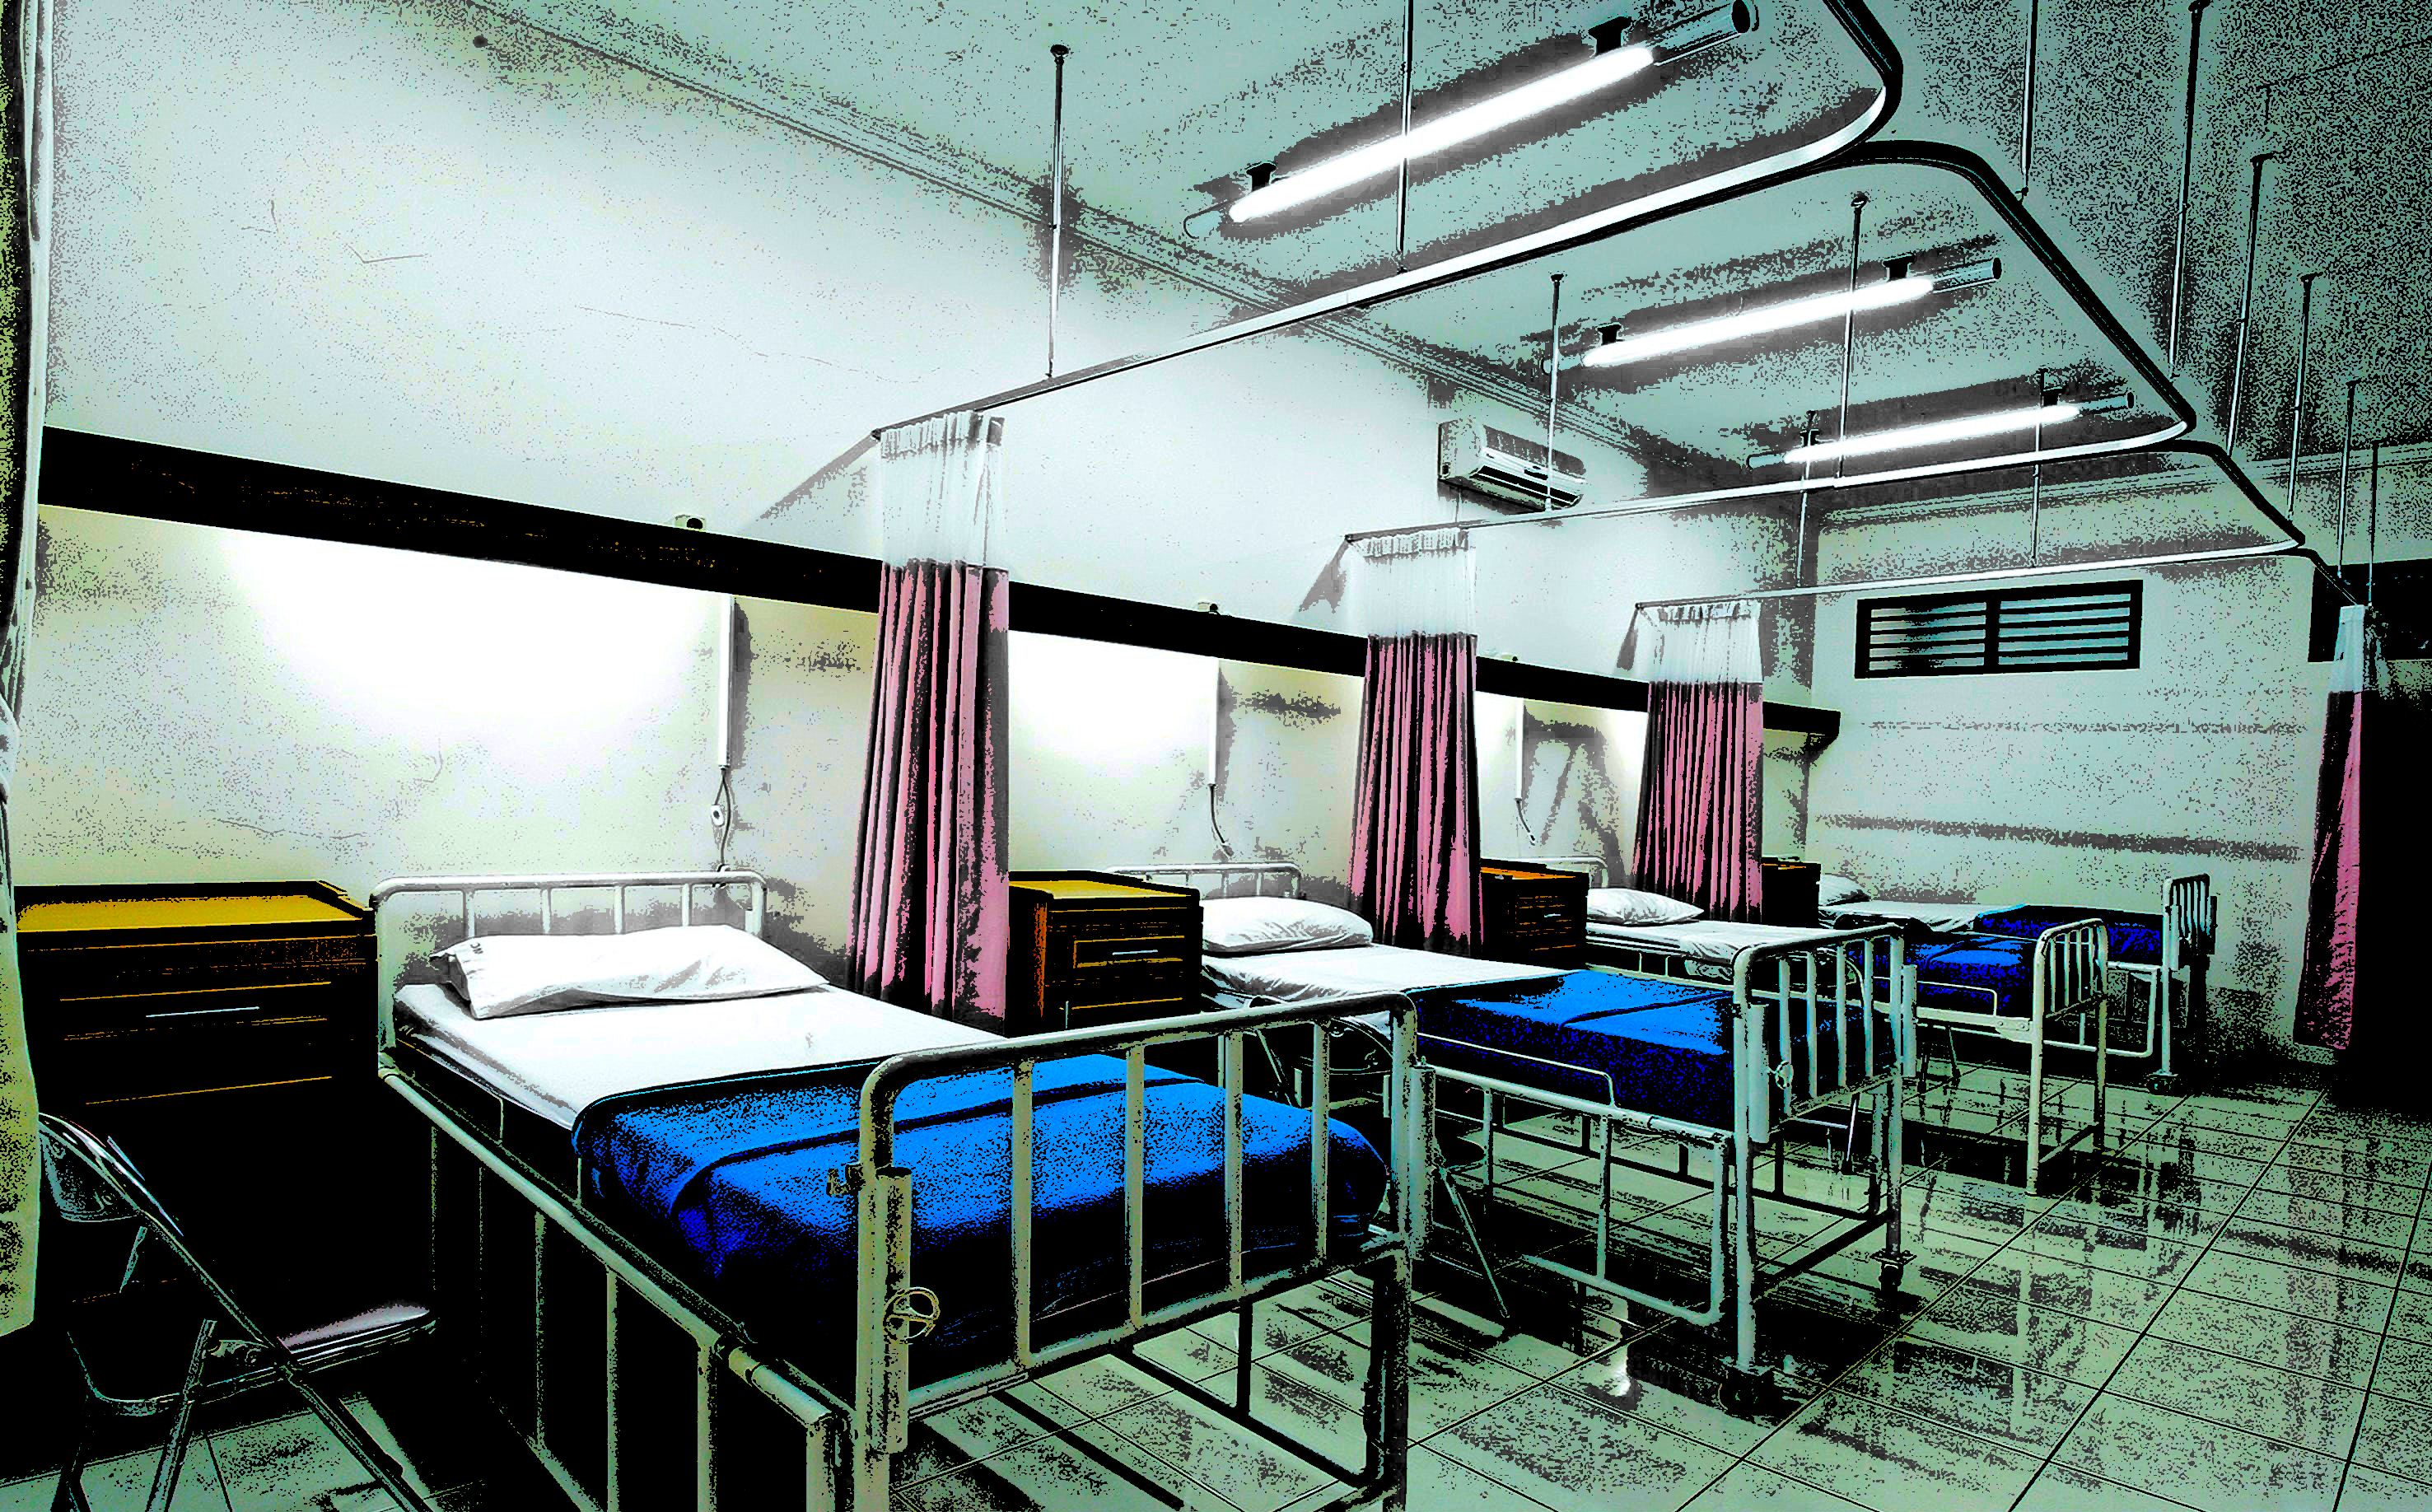
\includegraphics[width=7.0cm, keepaspectratio]{resources/img/wakeup-room.png}%
  \caption{Wakeup Room}
\end{figure}

This is where our protagonists are being brought to from the third floor and then subsequently wake up. First just feeling a
tingle in their body which goes away and then a wave hits all of them (triggered by Joanna starting to experiment on Dean, and
torturing someone loved by her), waking them up - Golab wants to disrupt her experiments, to make her more miserable.Joanna is
somewhat aware that something happened but focusses on "waking up" Dean. Surprisingly the experiments have reversed the muscular
atrophy and the protagonists feel quite healthy despite having been in a coma.

There is a nightstand next to everyone's bed with their regular street clothes and anything their relationship would have been
stashing in here.

There is a washing room with a toilet, shower and sink with mirror, which can be used for looking at the back to see the tattoo or
for the GM to trigger~\bluebf{Disadvantage} rolls for Nightmares or the like.

\gmnote{In one of my playtests I had a player with Nightmares, see encounter a single moth in the bathroom bumping against the
light, and later on a lot more whenever they found a reflective surface - tying the Disadvantage to the "Moth child".}

At the end of each bed is a medical file with a complete documentation of all the \textbf{medical} procedures, that includes a
\textbf{massive tattoo} in the shape of a symbol, which someone versed in lore would recognise as the symbol of the Death Angel
Golab.

\begin{figure}[!htbp]
  \centering
  \includegraphics[width=4.0cm]{resources/img/golab.png}
  \caption{Tattoo~\cite[p.~215]{KULT:core}}
\end{figure}

\gmnote{%
  In my play-tests I had the mother of the criminal put a bottle of good red wine, cutlery and a plate and a chequered napkin
  as a improvised table cloth in there.  Letter openers, knives pen, paper, newspapers with crossword puzzles.  Basically
  anything that would have been used in the opening scene or what the archetype would plausibly have.  All mobile phones have
  just a bit of battery left and just one bar of reception, if the close relationships are asleep they can be called in
  their dreams, but there is a lot of static on the call and they will expose the person they call to the influence of
  \textbf{Inferno} or \textbf{Limbo}~\cite[p.262]{KULT:core}.

  The mirror I used with great success to let moths (foreshadowing the \textbf{Moth Child}~\cite[p.~270]{KULT:core})
  appear, since the prolonged comatose sleep has brought the patients closer to \textbf{Limbo}.%
}

\subsubsection{Corridors}%
\label{ssub:Corridors}
The corridors have neon lights with motion sensors, when they wake up everything is dark outside, and the lights turn on
wherever they walk, with that unnerving ‘\textit{tick-tick-humm}’ that neon lights tubes do.  The walls have a few art prints of
a painter named ”Guy Vauquelin”\footnote{which you can use to tie it to the published scenario “The Atrocity Exhibition”
in~\cite[p.~94]{KULT:taroticum}}, and there are some indoor plants that are surprisingly well kept and alive.  Apart from that
I always ran this as an empty hospital, but, depending on the lines and veils of your players, you can go hog wild here and add
bloodstains, debris, mutilated and corpses drained of blood, signs of fight and struggle.  And since this is a pocket of reality
inside Inferno, you can make the walls move and ripple while you hear the sound of people from the other side of the veil or
children playing on a playground from the dream of one of the still comatose patients.

\subsubsection{Lifts}%
\label{ssub:lifts}

They will fall into their shafts the first time they are visited door closes, and then they reappear as if nothing happened
roll to \bluebf{Keep it Together (+Willpower)}.

If player's try to use them they will just fall through the floor.  Let them roll to \bluebf{Avoid Harm (+Reflexes)} to catch
themselves.  If they fail, they will fall down and back into the lift on the 5\textsuperscript{th} floor (because space is
just an illusion) and suffer \KULTred{1 harm} which they can roll to \bluebf{Endure Injury (+Fortitude)} for.

If player's decide to climb up or down, let them roll to \bluebf{Avoid Harm (+Reflexes)}, to avoid the lift hitting them from
above.  If they fail, they will fall down same as above.

Regardless of what they do, they will always end up on floor 5.

\subsubsection{Emergency Exits (\faLock)}%
\label{ssub:emergency_exits}

All exits are barricaded and warded by \hyperref[ssub:joanna_o_banion]{Joanna O'Banion} against intruders from \textbf{Inferno}.
If players try to see through the illusion close to any exit the will see some of the citizens or the shadow of the
\textbf{Black Citadels}~\cite[p.316]{KULT:core}.

They can break off the leg of a chair or take an IV stand pole which make up the barricade as a makeshift weapon.

\subsubsection{Other patient rooms: 503}%
\label{ssub:other_patient_rooms_503}

Room 503 is listed three times on the map\footnote{which was done by mistake originally}, and it has 2 patients a catholic priest
Paolo de Coppi, and a mayor Colin Malone. There's a newspaper on Colin's bedstand from 1953 about a car accident involving those
two in a small town close to Chicago, looking further one of the pictures shows Joanna in the background.

Where the rightmost room is pristine and tidy, though decorated in a distinct 1950s style. The second room in the middle is filled
with cobwebs as about 30 years have passed and the bodies are mummified almost wax-like. The leftmost room is filled with dust of
decades that have passed - the bodies are withered but still recognizable.

All changes in the "past" rooms will affect the rooms in the future, the realization of that should trigger a\bluebf{Keep it
Together (+Willpower)}.

\subsubsection{Other patient rooms: 50x}%
\label{ssub:other_patient_rooms}
These rooms are filled with other comatose patients.  Since Joanna O'Banion is a very diligent scientist as well as a skilled
alchemist, some of the patients will share a (uncanny) likeness with our protagonists.  These are the “control group” to make
sure that scientific/alchemistic discovery is not left to coincidence and is reproducible.

If one the protagonists die they may try to roll for \bluebf(Engage in Combat (+Violence)) to take over one of those comatose
bodies.

\begin{description}
  \item[On a (\KULTred{15+})] they can occupy the new body.  For the changed physicality let them change two of their active
        attributes.
  \item[On a (\KULTred{10--14})] they can share a new body with the current soul that is in there.  I used Sophie Liu (24), a
    talented climber, who had an accident (see p.~\pageref{ssub:other_patients}).  She's very vocal about her not liking the
    sharing of her body, which is something nobody else can hear.
  \item[On a (\KULTred{-9})] they share the body with Sophie, but they suffer another \redbf{-1 Stability}, and get a new
        disadvantage \hyperref[disadv:cannibalism]{cannibalism}~(p.~\pageref{disadv:cannibalism}).
\end{description}

\gmnote{%
  During playtest, the player who rolled a mixed success on this did great RP adding only his half of the conversation
  occasionally. And depending on how difficult things should be you can add some penalty for Sophie acting against the PCs will of
  doing or not doing something.
}

In any case the tattoo found on their original body will soon show up soon on the new body's back as well, it is not their body
but their soul that is trapped here.

\gmnote{%
  During playtest I had one PC with the hacker advantage use that skill while standing on the "magic circle" in the end to upload
  their consciousness to \goldbf{Limbo}, and leave their body behind and thusly escaping this place.
}

As far as the protagonists can see the control group has endured the same \textbf{medical} procedures, but none of the
“experimental” stuff.

\subsubsection{Staff Room (\faLock)}%
\label{ssub:staff_room}

This room is locked, but the key can be found with the \hyperref[ssub:orderly]{orderly}~(p.~\pageref{ssub:orderly}).  Also the
criminal~(p.~\pageref{sub:the_criminal}) can use their advantage of \bluebf{Burglar}, or someone can try to force the door open
by \bluebf{Engaging in Combat (+Violence)}, this last option will always be loud and get the attention of the orderly.

Inside the room there is
\begin{description}
  \item[a bunch of lockers] on the left wall, the blue colour is peeling off and you can see the rust.  There is a pistol and 2
        magazines inside~(see p.~\pageref{pistol}).
  \item[a working fridge] with a big green puddle.  The door is slightly ajar and inside there is a lot of mouldy food,
        the source of the puddle, and three beautiful roses.
  \item[a old computer with CRT monitor] on it there is a bunch of snuff porn and some searches about ‘torment’, there is a
        site about gruesome deaths in the internet explorer history, as well as some scanned pages containing weird (alchemical)
        symbols.  Reason why Joanna was using this computer for research is that only here the internet connection is working.  The
        protagonists can send emails to the outside world, but everything will take a while, and everything is old.
  \item[a kitchenette] used and some chairs and a crappy table, if someone tries to \bluebf{See through the Illusion (+Soul)}
        there are people moving through the room, staff from the other side of the veil.
\end{description}

\subsubsection{Laboratory (\faLock)}%
\label{ssub:laboratory}

The lab is a tidy room, the shelves are nicely sorted and the bottles of various chemicals are neatly labelled.  In the corner there
is a locked fridge with a glass door filled with medical samples, some of them being blood samples some filled with pale yellow liquor
samples, some of them labelled with the protagonists' names as well as some bar-code.See~(p.~\pageref{ssub:vials}) for more info on those.

In the bottom half there is a stash of opiate based pain killers requiring a \redbf{Disadvantage roll} for \redbf{Drug Addicts}, also
there is a bag of 12 black polished rocky dodecahedrons (whiskey stones).  And two bottles of white wine from 1912 with a worn label
referencing this as custom made for “RMS T\_t\_\_\_c”\footnote{RMS Titanic}.
\todo[inline]{fill me}

\subsubsection{Reception}%
\label{ssub:reception}

In my game the reception never came up as a meaningful location I kept it as a backup solution for the \textbf{staff room} so
instead of breaking open the door of the staff room I would still let the players do an \bluebf{Observe the situation (+Perception)}
or \bluebf{Investigate (+Reason)} to find the \textbf{pistol}.  There is a computer and some drawers where the protagonists might
find the \textbf{master keys/ID card}.

\subsubsection{The Office (\faLock)}%
\label{ssub:the_office}

This is where \hyperref[ssub:joanna_o_banion]{Joanna O'Banion} has her “Lair”, it is filled with a few workstations which all
don't work she has to light the office with candles, though the purple glow of the magic circle carved into the ground and
inlaid with tin does provide a bit of illumination in the back of the room.


\subsubsection{Other Rooms}%
\label{ssub:other_rooms}

\begin{itemize}[noitemsep]
  \item Toilets
  \item Waste Room (\faLock)
  \item Conference Room
  \item Cleaning Supply Room (\faLock)
\end{itemize}

These rooms are just set dressing, I have not planned anything with them, but feel free to introduce new and terrible surprises
for your players in here.

\subsection{Escape}%
\label{sub:escape}

There are two intended ways to escape from “The Ward”, adjust them to your game as needed.

\subsubsection{Option 1}%
\label{ssub:escape_option1}
One character willingly staying with Dean or Joanna will end the scenario and catapult the other characters out of
\textbf{Inferno} into their own bodies in the hospital, but not to the comatose ward from the opening scene, but one floor
above where they were brought to, which is now a regular sleep study station.  They are standing around clad in hospital gown,
where the nearest doctor or nurse will notice them and bring them to their room one floor below, which they have apparently
never left.

\subsubsection{Option 2}%
\label{ssub:escape_option2}
There is a binding circle in the laboratory.  The room is locked, but the door can be forced open or the PCs can use the staff
keys found on the \hyperref[ssub:orderly]{orderly}.  Stepping into the circle without preparation will cause its magic to
violently interact with the magic of the binding circle on the PCs back, dealing \KULTred{3 Harm} to \bluebf{Endure Injury
  (+Fortitude)}.  Using whatever they find in the lab or otherwise they can try to roll \bluebf{Engage in Combat (+Violence)} to
destroy the circle.

\begin{description}
  \item[On a (\KULTred{15+})] they will escape successfully.
  \item[On a (\KULTred{10--14})] there is a price to be paid, they leave something behind.
  \item[On a (\KULTred{-9})] the GM chooses one of
        \begin{itemize}[noitemsep]
          \item they cannot escape and have to stay as the pet of Joanna and Dean.
          \item they leave their body in \textbf{Inferno}, but return as a disembodied soul.
          \item they have to exchange someone from \textbf{Elysium}~\cite[p.~224]{KULT:core} to take their position here.
        \end{itemize}
\end{description}

\subsection{Home}%
\label{sub:home}

To close this scenario and tie in with the opening scene, I end the game with an improvised scene playing one year after the
last scene.  You can tie in the personal relations and extrapolate what might have happened to them in a year after the wake up.
In my play tests I made the relation of the people who stayed behind, start looking for clues where the PC went.  Ultimately
seeking out the other PCs for help, or explanation, after all they were also comatose in the same ward.

Characters who were left behind will be playing a game of cat and mouse with Dean\index{Moran, Dean}, maybe getting killed and
resurrected just to be chased and tortured another day, you can hint that they managed to escape \textbf{Inferno} after a few
years.

\clearpage % }}}
